\documentclass[10pt]{beamer}

\usetheme[progressbar=frametitle]{metropolis}
\usepackage[spanish, es-tabla]{babel} % Idioma español
\usepackage{appendixnumberbeamer}

\usepackage{booktabs}
\usepackage[scale=2]{ccicons}

\usepackage{pgfplots}
\usepgfplotslibrary{dateplot}
\usepackage[usenames,dvipsnames]{xcolor}

\usepackage{xspace}
\newcommand{\themename}{\textbf{\textsc{metropolis}}\xspace}

\title{Energ\'ias renovables en la generaci\'on el\'ectrica en Colombia}
\subtitle{An\'alisis exploratorio}
% \date{\today}
\date{}
\author{Alba L\'opez \and Ulises Linares \and Luis Bertel}
\institute{Inteligencia Artificial - Nivel Exploratorio}
\titlegraphic{\hfill\includegraphics[height=1.5cm]{logo.pdf}}

\begin{document}
	
	\maketitle
	
	\begin{frame}{Tabla de contenido}
		\setbeamertemplate{section in toc}[sections numbered]
		\tableofcontents%[hideallsubsections]
	\end{frame}
	
	\section[Contexto del problema]{Contexto del problema}
	
	\begin{frame}[fragile]{Retos de Colombia en cuanto a generaci\'on de energ\'ia}
		
Colombia se encuentra en una etapa clave de transformación de su matriz energética, impulsada por la necesidad de
diversificar las fuentes de generación eléctrica, reducir la dependencia de recursos hidroeléctricos y fósiles, y avanzar hacia un sistema energético más sostenible y resiliente frente al cambio climático. Históricamente, el país ha contado
con una alta participación de la generación hidroeléctrica —superior al 60 % en varios años—, lo cual ha permitido
mantener una baja intensidad de emisiones de carbono en el sector eléctrico en comparación con otras economías
de América Latina y el mundo. No obstante, esta dependencia ha expuesto al sistema a riesgos asociados con la
variabilidad climática, especialmente durante los períodos de sequía causados por fenómenos como El Niño, que
comprometen la estabilidad del suministro energético.

	\end{frame}
	
	\begin{frame}[fragile]{Objetivo espec\'ifico}
		
Analizar la evolución y el aporte de las fuentes de energía renovable en la generación eléctrica en Colombia entre los
años 2010 y 2025, con base en datos estadísticos comparativos, a fin de identificar tendencias, avances y desafíos en
el marco de la transición energética del país.
		
	\end{frame}
	
	\begin{frame}[fragile]{Pregunta orientadora}
		
¿Cómo ha evolucionado el aporte de las energías renovables en la generación eléctrica en Colombia entre 2014 y 2025,
y qué factores explican su desempeño?
		
	\end{frame}
	
	
	\section[Materiales y m\'etodos]{Materiales y m\'etodos}
	
		\begin{frame}[fragile]{Enfoque metodológico}
		
Este estudio se enmarca dentro del ciclo de vida de un proyecto de Machine Learning, específicamente en las etapas
de adquisición de datos, limpieza, análisis exploratorio, visualización, análisis multidimensional y modelos predictivos. Se adoptan herramientas y metodologías propias de la ciencia de datos para estructurar un análisis riguroso, reproducible y orientado a la extracción de conocimiento a partir de datos energéticos. El enfoque se limita exclusivamente al caso de Colombia \cite{Gacia}.
		
	\end{frame}
			
	
	\begin{frame}[fragile]{Conjunto de datos}
		
		El análisis se basa en un conjunto de datos inicialmente obtenido desde el portal Kaggle, el cual contiene información
		mensual de generación eléctrica clasificada por tipo de fuente energética, país, año y mes, expresada en gigavatios-
		hora (GWh). Esta base cubre el período comprendido entre 2010 y 2022. Para extender el alcance temporal hasta
		2025, se aplicaron técnicas de web scraping sobre fuentes oficiales y sitios especializados, lo que permitió actualizar
		el conjunto de datos con los registros más recientes disponibles.
		El dataset final fue consolidado y almacenado en formato CSV, lo cual facilitó su manipulación y análisis mediante
		herramientas de programación. Se realizó una curaduría manual y automatizada para garantizar la coherencia, 
		completitud y calidad de los datos utilizados.		
	\end{frame}
	
	\begin{frame}[fragile]{Detalle del conjunto de datos}
\begin{table}[h!]
	\begin{tabular}{|l|p{7cm}|}
		\hline
		\textbf{Variable}  & \textbf{Descripción}                                                                                                    \\ \hline
		COUNTRY            & Nombre del país al que corresponde el registro.                                                                         \\ \hline
		CODE\_TIME         & Código temporal en formato abreviado que indica el mes y año (por ejemplo, JAN2010).                                    \\ \hline
		TIME               & Representación en texto del mes y año (por ejemplo, January 2010).                                                      \\ \hline
		YEAR               & Año correspondiente al registro.                                                                                        \\ \hline
		MONTH              & Mes correspondiente al registro, en formato numérico (1–12).                                                            \\ \hline
		MONTH\_NAME        & Nombre del mes correspondiente al registro.                                                                             \\ \hline
		PRODUCT            & Tipo de fuente energética utilizada para la generación eléctrica (e.g., Hydro, Wind, Solar, etc.).                      \\ \hline
		VALUE              & Cantidad de electricidad generada en gigavatios-hora (GWh).                                                             \\ \hline		
	\end{tabular}
	\caption{Categorias del conjunto de datos}\label{table:tab1}
\end{table}	
	\end{frame}
	
		\begin{frame}[fragile]{Detalle del conjunto de datos - continuaci\'on}
		\begin{table}[h!]
			\begin{tabular}{|l|p{7cm}|}
				\hline
				\textbf{Variable}  & \textbf{Descripción}                                                                                                    \\ \hline				
				DISPLAY\_ORDER     & Indicador numérico utilizado para el ordenamiento visual de los productos.                                              \\ \hline
				yearToDate         & Acumulado de generación eléctrica en GWh desde el inicio del año hasta el mes actual.                                   \\ \hline
				previousYearToDate & Acumulado de generación eléctrica para el mismo periodo del año anterior.                                               \\ \hline
				share              & Porcentaje de participación del producto en la generación total del país (en formato decimal, por ejemplo 0.12 = 12\%). \\ \hline
			\end{tabular}
			\caption{Categorias del conjunto de datos}\label{table:tab2}
		\end{table}	
	\end{frame}
	
	\begin{frame}[fragile]{Herramientas tecnol\'ogicas}
		El procesamiento y análisis de los datos se llevaron a cabo en el lenguaje de programación Python, utilizando el entorno Jupyter Notebook por su versatilidad en la integración de código, visualizaciones y documentación. Las principales bibliotecas empleadas fueron:
		
		\begin{itemize}
			\item \textbf{Pandas:} para la manipulación y estructuración tabular de los datos.
			\item \textbf{NumPy:} para el manejo de operaciones numéricas.	
			\item \textbf{Matplotlib y Seaborn:} para la creación de visualizaciones descriptivas y comparativas.		
			\item \textbf{Scikit-learn}: para métodos de reducción de dimensiones, como PCA.
		\end{itemize}
	\end{frame}
	
		\begin{frame}[fragile]{Proceso metodol\'ogico (1)}
		\begin{enumerate}
			\item Adquisición y consolidación de datos:
			\begin{itemize}
				\item Descarga inicial del dataset desde Kaggle.		
				\item Actualización de datos mediante técnicas de web scraping para ampliar el rango temporal hasta 2025.		
				\item Fusión de fuentes y estandarización del formato general.		
			\end{itemize}
			\item Limpieza de datos:
			\begin{itemize}
				\item Revisión de datos faltantes, valores atípicos o inconsistentes.
				\item Conversión de tipos de datos y normalización de etiquetas (por ejemplo, estandarización de nombres de fuentes energéticas).
				\item Filtro de registros para conservar únicamente la información correspondiente a Colombia.
			\end{itemize}
			\item Análisis exploratorio de datos (EDA):
			\begin{itemize}
				\item Estadísticas descriptivas generales sobre la generación eléctrica total y por tipo de fuente.		
				\item Evaluación de la evolución temporal de la participación de energías renovables frente a no renovables.
			\end{itemize}			
		\end{enumerate}
	\end{frame}
	
	\begin{frame}[fragile]{Proceso metodol\'ogico (2)}
		\begin{enumerate}			
			\item[4.] Visualización de tendencias:
			\begin{itemize}
				\item Representación gráfica de series temporales, porcentajes de participación, acumulados anuales y estacionales.		
				\item Comparación de patrones interanuales y detección de puntos de inflexión relevantes.
			\end{itemize}
			\item[5.] Análisis multidimensional:
			\begin{itemize}
				\item Aplicación de técnicas para explorar las relaciones entre variables como tipo de generación, volumen mensual, variabilidad estacional, y evolución anual.		
				\item Uso de gráficos de calor, diagramas de dispersión múltiple o métodos de reducción de dimensiones (como PCA), en caso de ser necesarios.
			\end{itemize}	
			\item[6.] An\'alisis supervisado y no supervisado:
			\begin{itemize}
				\item An\'alisis de tendencia usando regresi\'on lineal.		
				\item Uso de cluster para agrupar generaci\'on por a\~no.
			\end{itemize}	
		\end{enumerate}
	\end{frame}
	
	
\section[Resultados]{Resultados}
	
\subsection{Análisis exploratorio}
	
\begin{frame}[fragile]{Estructura de datos utilizada}
\begin{verbatim}
<class 'pandas.core.frame.DataFrame'>
Index: 3104 entries, 46557 to 212133
Data columns (total 4 columns):
#   Column   Non-Null Count  Dtype  
---  ------   --------------  -----  
0   YEAR     3104 non-null   int64  
1   MONTH    3104 non-null   int64  
2   PRODUCT  3104 non-null   object 
3   VALUE    3104 non-null   float64
dtypes: float64(1), int64(2), object(1)
memory usage: 121.2+ KB
\end{verbatim}
\end{frame}
		
\begin{frame}[fragile]{Cantidad de energía clasificada según tipo}
\begin{figure}[t]
	\centering
	\includegraphics[width=0.6\linewidth]{../../reports/fig_3}
	\caption{Cantidad de energ\'ia clasificada por tipo}
	\label{fig:fig3}
\end{figure}
\end{frame}
	
\begin{frame}[fragile]{Evolución de la producción neta de energía en Colombia}
\begin{figure}[t]
	\centering
	\includegraphics[width=0.7\linewidth]{../../reports/fig_4}
	\caption{Evolución de la producción neta de energía en Colombia}
	\label{fig:fig4}
\end{figure}
\end{frame}
	
\begin{frame}[fragile]{Producción neta mensual de energía en Colombia}
	\begin{figure}[t]
		\centering
		\includegraphics[width=0.7\linewidth]{../../reports/fig_5}
		\caption{Producción neta mensual de energía en Colombia}
		\label{fig:fig5}
	\end{figure}
\end{frame}

\begin{frame}[fragile]{Matriz energética de Colombia}
\begin{verbatim}
PRODUCT
Hydro          601415.683695
Natural gas    153592.481385
Coal            71158.873666
Others          31527.442435
Solar            7138.600132
Wind              629.372654
Nuclear             0.000000
Name: VALUE, dtype: float64
\end{verbatim}
\end{frame}

\begin{frame}[fragile]{Matriz energética de Colombia}
\begin{figure}[t]
	\centering
	\includegraphics[width=1.2\linewidth]{../../reports/fig_6}
	\caption{Matriz energética de Colombia}
	\label{fig:fig6}
\end{figure}	
\end{frame}


\begin{frame}[fragile]{Energía según tipo de generación}
\begin{figure}[t]
	\centering
	\includegraphics[width=0.9\linewidth]{../../reports/fig_7}
	\caption{Energía según tipo de generación}
	\label{fig:fig7}
\end{figure}	
\end{frame}


\begin{frame}[fragile]{Evolución de la producción de energía en Colombia según tipo de generación}
\begin{figure}[t]
	\centering
	\includegraphics[width=0.9\linewidth]{../../reports/fig_8}
	\caption{Evolución de la producción de energía en Colombia según tipo de generación}
	\label{fig:fig8}
\end{figure}	
\end{frame}
	
	
\begin{frame}[fragile]{Evolución de la producción de energía en Colombia según tipo de generación}
\begin{figure}[t]
	\centering
	\includegraphics[width=0.9\linewidth]{../../reports/fig_9}
	\caption{Evolución de la producción de energía en Colombia según tipo de generación}
	\label{fig:fig9}
\end{figure}	
	\end{frame}
	
		\begin{frame}[fragile]{Proporción energía renovables vs No renovables}
\begin{figure}[t]
	\centering
	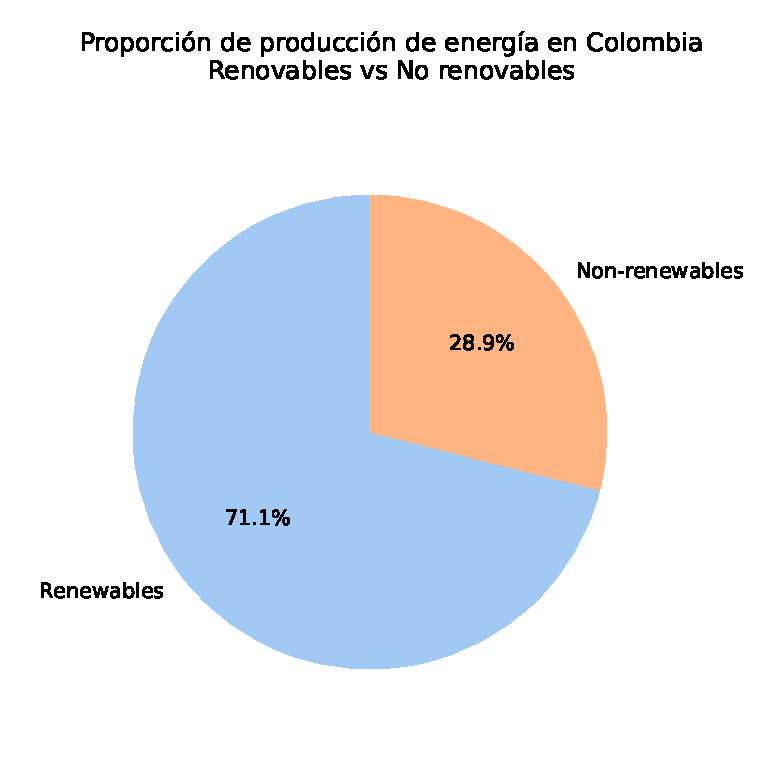
\includegraphics[width=0.6\linewidth]{../../reports/fig_10}
	\caption{Proporción de producción de energía en Colombia Renovables vs No renovables}
	\label{fig:fig10}
\end{figure}	
\end{frame}
	
	
\begin{frame}[fragile]{Evolución energía renovable vs no renovable (2014-2025)}
\begin{figure}[t]
		\centering
		\includegraphics[width=0.9\linewidth]{../../reports/fig_11}
		\caption{Evolución de la producción de energía en Colombia. Renovable vs no renovable (2014-2025)}
		\label{fig:fig11}
\end{figure}
\end{frame}
	
\begin{frame}[fragile]{Producción de energía de fuentes Renovables}
\begin{figure}[t]
	\centering
	\includegraphics[width=1\linewidth]{../../reports/fig_12}
	\caption{Producción de energía de fuentes Renovables}
	\label{fig:fig12}
\end{figure}
\end{frame}
	
\begin{frame}[fragile]{Evolución energía de fuentes renovables (2014-2025)}
\begin{figure}[t]
			\centering
			\includegraphics[width=0.9\linewidth]{../../reports/fig_13}
			\caption{Evolución de la producción de energía en Colombia. Fuentes Renovables (2014-2025)}
			\label{fig:fig13}
\end{figure}
\end{frame}
	
\begin{frame}[fragile]{Producción de energía de fuentes Renovables No hidraulica}
\begin{figure}[t]
		\centering
		\includegraphics[width=0.7\linewidth]{../../reports/fig_14}
		\caption{Producción de energía. Fuentes Renovables. No hidraulica}
		\label{fig:fig14}
\end{figure}
\end{frame}
	
\begin{frame}[fragile]{Evolución energía de fuentes Renovables No hidraulica}
\begin{figure}[t]
	\centering
	\includegraphics[width=1\linewidth]{../../reports/fig_15}
	\caption{Producción de energía. Fuentes Renovables. No hidraulica}
	\label{fig:fig15}
\end{figure}
\end{frame}
	
\begin{frame}[fragile]{Producción de energía de fuentes no renovables}
\begin{figure}[t]
			\centering
			\includegraphics[width=0.9\linewidth]{../../reports/fig_16}
			\caption{Producción de energía de fuentes no renovables}
			\label{fig:fig16}
\end{figure}
\end{frame}
	
\begin{frame}[fragile]{Evolución energía en Colombia de fuentes no renovables (2014-2025)}
		\begin{figure}[t]
			\centering
			\includegraphics[width=0.7\linewidth]{../../reports/fig_17}
			\caption{Evolución de la producción de energía en Colombia de fuentes no renovables (2014-2025)}
			\label{fig:fig17}
\end{figure}
\end{frame}
	
\subsection{Análisis supervisado}
	
\begin{frame}[fragile]{Regresión lineal de la producción eléctrica en Colombia}
\begin{figure}[t]
			\centering
			\includegraphics[width=0.7\linewidth]{../../reports/fig_18}
			\caption{Regresión lineal de la producción eléctrica en Colombia}
			\label{fig:fig18}
\end{figure}
\end{frame}
	
\subsection{Análisis no supervisado}
	
\begin{frame}[fragile]{Clustering de años según patrón energético (PCA + KMeans)}
\begin{figure}[t]
			\centering
			\includegraphics[width=0.9\linewidth]{../../reports/fig_19}
			\caption{Clustering de años según patrón energético (PCA + KMeans)}
			\label{fig:fig19}
\end{figure}
\end{frame}
	
\section[Conclusiones]{Conclusiones}
	
\begin{frame}{En resumen}
\begin{itemize}
		\item La generación hidroeléctrica domina ampliamente entre las fuentes renovables.
		\item Las fuentes como solar y eólica aún representan un porcentaje muy bajo, aunque con potencial de crecimiento.
		\item La energía basada en fósiles también tiene un peso relevante, especialmente el gas natural.
		\item Se observa un crecimiento sostenido de la producción entre 2014 y 2018.
		\item El análisis completo de 2019 a 2025 permitirá ver el impacto de políticas o proyectos recientes.
\end{itemize}
\end{frame}
		
	
\begin{frame}[standout]
	¿Preguntas?
\end{frame}
	
\begin{frame}[allowframebreaks]{Bibliografía}						
	\bibliographystyle{apalike}
	\bibliography{suministros_eficientes.bib}		
\end{frame}
	
\end{document}